\documentclass[10pt,twocolumn]{article}
\usepackage[margin=0.55in,top=0.58in,bottom=0.58in]{geometry}
\usepackage{amsmath,amssymb,amsthm}
\usepackage{booktabs}
\usepackage{graphicx}
\usepackage{microtype}
\usepackage[hidelinks]{hyperref}
\usepackage{xurl}

\raggedbottom
\setlength{\columnsep}{0.20in}
\setlength{\parskip}{1.4pt}
\setlength{\textfloatsep}{7pt plus 2pt minus 2pt}
\setlength{\dbltextfloatsep}{8pt plus 2pt minus 2pt}

\title{\vspace{-1.2em}\textbf{Mito-Polaritons Meet the Resource Boundary: Exact Hopfield $A^2$ Invariants, Thermodynamic Maintenance Horizons, and Constructive Lean~4 Certificates for the 71-THz Mitochondrial Quantum State}\vspace{-0.4em}}
\author{Lluis Eriksson\\
\small Independent Researcher (\nolinkurl{https://github.com/lluiseriksson})\\
\small Operational Synthesis Connecting \texttt{ARR-2025-2AQXS44H6Z8GQAG2} and \texttt{bioRxiv:2026.09.10.750628v1}\vspace{-0.6em}}
\date{November 26, 2026}

\begin{document}
\maketitle

\begin{abstract}
\noindent In September~2026, Yang, Gu, and Song (\texttt{bioRxiv:10.64898/2026.09.10.750628v1}) reported an anomalous $71.0$-THz mid-infrared oscillation mode unique to living cells and intact mitochondrial cristae, modeling it as a lipid $\text{CH}_2$ vibrational polariton (``mito-polariton'') splitting the $87$-THz $\text{CH}_2$ stretch into $71$~THz and $103$~THz branches and showing $\sim 10\%$ ATP modulation under weak resonant irradiation. Here we apply our previously published operational coherence-maintenance and resource-boundary framework (\texttt{ARR-2025-2AQXS44H6Z8GQAG2}, Dec.~2025 / Jul.~2026, and its 2025--2026 AIRR.SCIENCE companion series) to audit the mito-polariton hypothesis quantitatively and derive sharp, falsifiable predictions backed by a zero-floating-point verification suite (\texttt{MITO-POLARITON-BOUND-CERT-1.0}) with 18 constructive Lean~4.35.0 theorems (0~\texttt{sorry}, 0~custom axioms, 0~\texttt{Classical.choice}), 16 canonical JSON certificates, and 30 unit/forgery/AST tests. Five exact results emerge: (i)~at $\nu_- = 71$~THz and $\omega_0 = 87$~THz, coupling enters the ultrastrong regime ($\eta = g/\omega_0 = 1264/6177 \approx 0.2046 > 0.1$), where the gauge-invariant Hopfield $A^2$ term (Thomas--Reiche--Kuhn sum rule $\nu_+\nu_-=\omega_0^2$) predicts an upper polariton at $\nu_+^{\mathrm{Hop}} = 7569/71 \approx 106.61$~THz---a $+3.61$~THz blue-shift over RWA's $103$~THz, directly testable in $\text{D}_2\text{O}$ where water's O--D stretch clears the $100$--$110$~THz window; (ii)~by our Conditional Maintenance Work Theorem at $T=310$~K ($k_B T \approx 26.71$~meV, $\Delta G_{\mathrm{ATP}}\approx 518.2$~meV), bulk-water picosecond dephasing ($\kappa_{\mathrm{bulk}}\sim 10^{12}\,\mathrm{s}^{-1}$) exceeds the entire mitochondrial ATP power budget ($P_{\mathrm{mito}}/k_B T \sim 1.94\times 10^6\,\mathrm{s}^{-1}$) by $5\times 10^5$, cleanly separating a zero-maintenance passive vacuum-dressed polariton (Regime~I, $C_\Delta=0$) from active non-equilibrium coherence (Regime~II, $C_\Delta>0$, requiring $\kappa_\downarrow \lesssim 2\times 10^6\,\mathrm{s}^{-1}$); (iii)~cristae collar suppression (\textsc{rip-u}) and spectral detuning into the $60$--$80$~THz quiet window suppress $\omega\neq 0$ decay but cannot remove an irreducible Davies $\omega=0$ pure-dephasing floor $\kappa_0$; (iv)~for $N$ bosonic $\text{CH}_2$ stretches in the vacuum regime ($\bar{n}_{\mathrm{th}} < 2\times 10^{-6}$ at $310$~K), coupling to one cavity mode splits the $N$ dipoles into $1$ bright mode and $N-1$ orthogonal dark modes with exact Hopfield lower-polariton matter weight $w_{\mathrm{mat}} = \nu_-^2/(\omega_0^2+\nu_-^2) = 5041/12610 \approx 0.3998 < 1/2$, forcing local vibrational dephasing to scatter into the dark manifold at rate $\Gamma_{\mathrm{MP}^-\to\mathcal{D}} = w_{\mathrm{mat}}\frac{N-1}{N}\gamma_{\mathrm{loc}}$ (zero $1/N$ collective protection against Markovian local dephasing), while an $S$-lamella coupled cristae stack outperforms factorized single-bilayer water-band shielding whenever $C_S(\delta+\beta)+r < 1$; and (v)~we deliver a four-test experimental falsification matrix separating classical artifacts, Regime~I, and Regime~II.
\end{abstract}

\section{Introduction, Scope, and Prior Program}
In December~2025 (revised July~2026), we formulated an operational resource-boundary program~\cite{Eriksson2025GeometryMembranes} (supported by~\cite{Eriksson2025MaintenanceWork,Eriksson2026RipUOmegaZero,Eriksson2026MaintenanceNotRestoration,Eriksson2026ManyBodyFilling,Eriksson2026PassiveNetworks}) connecting three layers: \emph{geometry} as cross-interface suppressibility, \emph{membranes} as engineered collars implementing upper-rate suppression (\textsc{rip-u}), and \emph{life} operationally as sustained maintenance of internal organization under finite thermodynamic power budgets. Nine months later, Yang, Gu, and Song~\cite{YangGuSong2026Mito} reported FTIR evidence for a $71.0$-THz ($2368\,\mathrm{cm}^{-1}$) mode present exclusively in living cells, intact tissues, and structurally preserved mitochondria, disappearing upon cristae disruption or drying, and linked via resonant $71$/$87$-THz irradiation to an approximate $10\%$ increase in cellular ATP production.

\paragraph{Scope and epistemic hygiene.}
We emphasize two strict boundaries. First,~\cite{YangGuSong2026Mito} is an \emph{unrefereed bioRxiv preprint} whose experimental claims await independent replication; we neither endorse nor assume its unverified biological conclusions, but rather apply exact algebraic and open-quantum-system theorems to extract hard physical constraints and falsifiable tests. Second, following~\cite{Eriksson2025GeometryMembranes}, our thermodynamic maintenance bounds are unconditional in the law-grade energy-pinching $\Delta$-track ($C_\Delta(\rho) = S(\rho\|\Delta[\rho])$) and explicitly conditional on approximate Petz/Pythagorean sufficiency~\cite{FawziRenner2015CMI} when lifted to general membrane coarse-grainings ($E$-track).

\section{Five Exact Theoretical Bridges}

\paragraph{1. Gauge-Invariant Hopfield $A^2$ Shift vs.\ Naive RWA.}
Yang, Gu, and Song~\cite{YangGuSong2026Mito} model the $71.0$-THz line as the lower polariton $\mathrm{MP}^-$ of lipid $\text{CH}_2$ stretches ($\omega_0 \approx 87$~THz) coupled to cristae-confined infrared modes, inferring a symmetric rotating-wave-approximation (RWA) upper branch $\nu_+^{\mathrm{RWA}} = 87 + 16 = 103$~THz hidden inside the $90$--$110$~THz $\text{H}_2\text{O}$/amide-A band. However, at resonant coupling $\omega_c = \omega_0$ with splitting $\Omega_R \gtrsim 32$~THz ($\eta = g/\omega_0 > 0.2$), RWA breaks gauge invariance and violates the Thomas--Reiche--Kuhn (TRK) sum rule~\cite{Hopfield1958Polariton,Rzazewski1975NoGo,FriskKockum2019USC}. Including the diamagnetic $A^2$ coefficient $D = g^2/\omega_0$, the exact Hopfield secular equation for $\lambda = \nu^2$ is
\begin{equation}
\label{eq:hopfield}
\lambda^2 - (\omega_c^2 + \omega_0^2 + 4g^2)\lambda + \omega_c^2\omega_0^2 = 0.
\end{equation}
At resonance ($\omega_c = \omega_0$),~\eqref{eq:hopfield} yields $\nu_+ \nu_- = \omega_0^2$ and $\nu_+ - \nu_- = 2g$ identically (Lean Thm.~1), with strictly positive discriminant $(\omega_c^2-\omega_0^2)^2 + 8g^2(\omega_c^2+\omega_0^2) + 16g^4 \ge 0$ preventing superradiant collapse (Thm.~2). Setting $\omega_0 = 87$~THz and $\nu_- = 71$~THz forces
\begin{equation}
\label{eq:shift}
\begin{aligned}
\nu_+^{\mathrm{Hop}} &= \frac{87^2}{71} = \frac{7569}{71} \approx 106.6056\,\mathrm{THz}, \\
\nu_+^{\mathrm{Hop}} - \nu_+^{\mathrm{RWA}} &= \frac{256}{71} \approx +3.61\,\mathrm{THz},
\end{aligned}
\end{equation}
and normalized coupling $\eta = g/\omega_0 = 1264/6177 \approx 0.2046 > 1/5$ (Thms.~3--4, Fig.~\ref{fig:fig1}). Because $\text{D}_2\text{O}$ shifts the water stretch from $\sim 102$~THz down to $\sim 74.9$~THz ($2500\,\mathrm{cm}^{-1}$), substituting $\text{D}_2\text{O}$ clears the $100$--$110$~THz window to directly resolve $103$~THz vs.\ $106.61$~THz, while $\text{CD}_2$ lipid deuteration shifts bare $\omega_0$ to $87/\sqrt{2} \in (61.5, 61.6)$~THz (Thm.~5).

\paragraph{2. Bioenergetic ATP Resource Horizon (Regime~I vs.\ Regime~II).}
By Theorem~4.1 and Theorem~9.1 of~\cite{Eriksson2025GeometryMembranes,Eriksson2025MaintenanceWork}, under battery-assisted thermal operations at bath temperature $T$ with Markovian thermal-fixed-point generator and rate floor $\dot{C}_{\Delta,\mathrm{loss}}(\rho) \ge \kappa_\downarrow(\epsilon) C_\Delta(\rho)$, sustaining coherence $C_\Delta(\rho) \ge C_0$ demands minimal continuous power
\begin{equation}
\label{eq:horizon}
P_{\mathrm{maint}}^\star(\rho) \ge k_B T\,\dot{C}_{\Delta,\mathrm{loss}}(\rho) \ge k_B T\,\kappa_\downarrow(\epsilon)\,C_0.
\end{equation}
At physiological $T = 310$~K ($k_B T \approx 26.71$~meV, $k_B T/h \approx 6.46$~THz), one ATP hydrolysis releases $\Delta G_{\mathrm{ATP}} \approx 50\,\mathrm{kJ/mol} \approx 518.2\,\mathrm{meV} \approx 19.40\,k_B T$ (while $h\cdot 71\,\mathrm{THz} \approx 293.63\,\mathrm{meV} \approx 11.0\,k_B T$, so $2\,h\nu_- \approx 587.3\,\mathrm{meV} > \Delta G_{\mathrm{ATP}}$, Thm.~9). Even allocating a mitochondrion's full flux $R_{\mathrm{ATP}} \sim 10^5\,\mathrm{ATP/s}$ gives $P_{\mathrm{mito}}/(k_B T) \approx 1.94\times 10^6\,\mathrm{s}^{-1}$. Consequently, bulk-water picosecond vibrational dephasing ($\kappa_{\mathrm{bulk}} \sim 10^{12}\,\mathrm{s}^{-1}$) exceeds the entire mitochondrial budget at $C_0=1$~nat by a factor of $5\times 10^5$ (Thms.~6--8, Fig.~\ref{fig:fig2}a). This proves a sharp operational dichotomy:
\begin{itemize}\itemsep 1pt
\item \textbf{Regime~I (Passive Vacuum-Dressed Polariton, $C_\Delta = 0$):} The $71$-THz mode is a stationary energy eigenstate of the cristae cavity. Its $\Delta$-track active coherence maintenance power is identically zero (Thm.~7); metabolic work maintains membrane geometry, not off-diagonal coherence.
\item \textbf{Regime~II (Active Non-Equilibrium Coherence, $C_\Delta > 0$):} Thermodynamically feasible at $C_0 \sim 1$~nat \emph{only} if cristae engineering suppresses the effective dephasing floor below $\kappa_\downarrow \lesssim 2\times 10^6\,\mathrm{s}^{-1}$ ($\tau_{\mathrm{coh}} \gtrsim 0.5\,\mu\mathrm{s}$). Moreover, by~\cite{Eriksson2026MaintenanceNotRestoration} (Thm.~10), periodic endpoint refresh ($W_0/T_{\mathrm{per}}\to 0$) must never be conflated with continuous holding under~\eqref{eq:horizon}.
\end{itemize}

\paragraph{3. Cristae Collar RIP-U vs.\ Irreducible $\omega = 0$ Davies Floor.}
Detuning $\nu_- = 71$~THz into the $60$--$80$~THz quiet gap moves three times further from the $95$-THz water/amide edge than bare $87$~THz ($\Delta_- = 24 = 3\Delta_0$), giving a Lorentzian bath-density suppression factor $(\Delta_-^2+\Gamma^2)/(\Delta_0^2+\Gamma^2) \ge 5$ whenever $\Gamma \le \Delta_0$ (Thm.~14). Simultaneously, the lipid bilayer collar enforces an upper-rate ceiling $\kappa_\uparrow(\epsilon) \le \kappa_0 + B_0 q^\epsilon$ (\textsc{rip-u},~\cite{Eriksson2025GeometryMembranes}). Yet by~\cite{Eriksson2026RipUOmegaZero} (Thms.~12--13, Fig.~\ref{fig:fig2}b), slow fluctuations of the membrane potential $\Delta\Psi_m$ at $\omega \simeq 0$ enter the Davies Dirichlet form~\cite{Davies1974Markovian} $\mathcal{E}^{(0)}_\sigma(O) = \frac{\gamma(0)}{2}\|[S(0),O]\|^2_{2,\sigma}$ (audited in Mode~3a via the equivalent GNS trace norm $\frac{\gamma_0}{2}\mathrm{Tr}(\sigma[S(0),O]^\dagger[S(0),O])$, matching KMS identically on maximally mixed $\sigma$ and sharing the exact vanishing condition $[S(0),O]=0$): whenever $S(0)$ distinguishes $\mathrm{MP}^\pm$ ($s_- \neq s_+$), $\kappa_\downarrow(\epsilon) \ge \kappa_0 > 0$ persists for \emph{every} collar thickness $\epsilon$, fixing an unremovable resource horizon.

\paragraph{4. Bosonic Dark-Mode Leakage and Lamellar Crista Stack Mapping.}
Coupling $N$ identical bosonic lipid $\text{CH}_2$ stretches $\{b_j\}_{j=1}^N$ ($\omega_0 = 87$~THz) uniformly ($g_0 = g/\sqrt{N}$) to one crista cavity photon mode $a$ isolates a single symmetric bright Dicke mode $B = N^{-1/2}\sum_{j=1}^N b_j$ and $N-1$ orthogonal dark modes $\mathcal{D}$ (Thm.~15). At physiological $T = 310$~K, $\hbar\omega_0/(k_B T) = h\cdot 87\,\mathrm{THz}/(k_B\cdot 310\,\mathrm{K}) \approx 13.47 > 13$, so the Bose--Einstein thermal occupation satisfies $\bar{n}_{\mathrm{th}} = (e^{\hbar\omega_0/k_B T}-1)^{-1} < 2\times 10^{-6}$ (true value $\approx 1.41\times 10^{-6}$, placing the lipid ensemble firmly in the vacuum/single-excitation bosonic regime, distinct from half-filled fermionic SSH chains~\cite{Eriksson2026ManyBodyFilling}). From the exact resonant Hopfield secular equation~\eqref{eq:hopfield} ($\nu_+\nu_- = \omega_0^2$), the lower polariton $\mathrm{MP}^-$ carries exact matter and photonic weights
\begin{equation}
\label{eq:filled}
\begin{aligned}
w_{\mathrm{mat}} &= \frac{\nu_-^2}{\omega_0^2 + \nu_-^2} = \frac{5041}{12610} \approx 0.3998 < \frac{1}{2}, \\
w_{\mathrm{phot}} &= \frac{\omega_0^2}{\omega_0^2 + \nu_-^2} = \frac{7569}{12610} \approx 0.6002,
\end{aligned}
\end{equation}
so the diamagnetic $A^2$ blue-shift tilts $\mathrm{MP}^-$ slightly photonic (Thm.~16, Fig.~\ref{fig:fig3}a). Under site-uncorrelated Markovian vibrational dephasing $\gamma_{\mathrm{loc}}\sum_{j=1}^N\mathcal{D}[b_j^\dagger b_j]$, each single-site excitation $|j\rangle = b_j^\dagger|0\rangle$ has overlap $|\langle B|j\rangle|^2 = 1/N$ with the bright mode and $1 - 1/N$ with $\mathcal{D}$, yielding exact bright-to-dark scattering rate $\Gamma_{B\to\mathcal{D}} = \gamma_{\mathrm{loc}}(1-1/N)$ and polariton-to-dark rate $\Gamma_{\mathrm{MP}^-\to\mathcal{D}} = w_{\mathrm{mat}}\frac{N-1}{N}\gamma_{\mathrm{loc}} \ge \frac{1}{2}w_{\mathrm{mat}}\gamma_{\mathrm{loc}}$ for every $N \ge 2$ (Thm.~15): unlike static inhomogeneous disorder (suppressed when $\sigma_\omega \ll \Omega_R$), local Markovian dephasing enjoys \emph{zero} $1/N$ collective protection as $N\to\infty$. Conversely, mapping a stack of $S$ lamellar mitochondrial cristae (spacing $20$--$40$~nm, coupled via crista junctions) directly to the passive multi-port filter tuple $(S, C_S, \delta, \beta, r)$ of~\cite{Eriksson2026PassiveNetworks}---with $S$ coupled bilayer cavities, passband tolerance $\delta$ across the $60$--$80$~THz quiet window, inter-crista junction loss defect $\beta$, $3(S-1)$ single-port tangential calibration constraints with singular-value constant $C_S$, and coupled-stack stopband transmittance $r$ across the $90$--$110$~THz water/amide band---Theorem~17 proves that whenever $C_S(\delta+\beta)+r < 1$, any factorized single-bilayer model suffers worst-case water-band leakage $\ge 1 - C_S(\delta+\beta) > r$ (Fig.~\ref{fig:fig3}b), explaining why intact multi-crista stacking is necessary for broadband shielding.

\section{Constructive Lean~4.35.0 Kernel and Zero-Float Audit}
We formalize all 18 algebraic and thermodynamic pillars in \texttt{lean/\allowbreak MitoPolaritonBoundCert.lean} under Lean~4.35.0 without Mathlib, audited via \texttt{\#print axioms} to depend strictly on \texttt{propext} and \texttt{Quot.sound} (0~\texttt{sorry}, 0~custom axioms, 0~\texttt{Classical.choice}, 0~warnings; Table~\ref{tab:lean}). Our standalone verifier \texttt{src/\allowbreak mito\_polariton\_bound\_verifier.py} enforces an AST-audited zero-float invariant (zero \texttt{float} literals, zero \texttt{float()} calls, zero \texttt{/} or \texttt{/=}, zero \texttt{math}/\texttt{numpy} imports). All 16 canonical certificates (\texttt{C01}--\texttt{C16}, Table~\ref{tab:certs}) pass \texttt{python -m} \nolinkurl{src.mito_polariton_bound_verifier} \texttt{certificates}, and all 30 unit/forgery/AST tests pass under \texttt{pytest -q}.

\begin{table*}[t]
\centering
\scriptsize
\setlength{\tabcolsep}{2.8pt}
\caption{All 18 constructive Lean~4.35.0 theorems in \texttt{MitoPolaritonBoundCert.lean} (0~\texttt{sorry}, 0~\texttt{Classical.choice}), with exact statements.}
\label{tab:lean}
\begin{tabular}{@{}cll@{}}
\toprule
\# & Lean Theorem Identifier & Exact Formalized Statement (over $\mathbb{Z}$ or $\mathbb{N}$) \\
\midrule
1 & \texttt{hopfield\_trk\_vieta\_invariants} & $\nu_+\nu_-=\omega_0^2 \wedge \nu_+-\nu_-=2g \implies \nu_+^2+\nu_-^2=2\omega_0^2+4g^2 \wedge \nu_+^2\nu_-^2=\omega_0^4$ \\
2 & \texttt{hopfield\_no\_superradiant\_instability} & $a,b,g^2\ge 0 \implies (a+b+4g^2)^2-4ab = (a-b)^2+8g^2(a+b)+16g^4 \ge 0$ \\
3 & \texttt{mito\_71\_87\_103\_rwa\_vs\_hopfield\_shift} & $71\cdot 103+16^2=87^2=7569;\ 10660\cdot 71<756900<10661\cdot 71;\ 7\cdot 71<2\cdot 256$ \\
4 & \texttt{mito\_ultrastrong\_coupling\_regime} & $7569-71^2=2528,\ 2\cdot 71\cdot 87=12354,\ \eta=1264/6177 > 1/5$ ($5\cdot 1264>6177$) \\
5 & \texttt{isotope\_cd2\_and\_d2o\_window\_clearance} & $2\cdot 615^2 < 870^2 < 2\cdot 616^2$ ($87/\sqrt{2}\in(61.5,61.6)$); $75<100<103<7569/71$ \\
6 & \texttt{maintenance\_power\_pythagorean\_split} & $k_BT,F_{\mathrm{diag}}\ge 0 \wedge k_BT\sigma\le P_{\min} \wedge \sigma=F_{\mathrm{diag}}+C_{\mathrm{loss}} \wedge \kappa_\downarrow C_0\le C_{\mathrm{loss}} \implies k_BT\kappa_\downarrow C_0\le P_{\min}$ \\
7 & \texttt{passive\_equilibrium\_zero\_coherence\_cost} & $k_BT,\kappa_0,C_0>0 \implies k_BT(\kappa_0\cdot 0)=0 \wedge 0 < k_BT(\kappa_0 C_0)$ (Regime~I vs.~II) \\
8 & \texttt{mito\_resource\_horizon\_five\_order\_gap} & $20\cdot 10^5 = 2\cdot 10^6 \wedge (5\cdot 10^5)\cdot(2\cdot 10^6)=10^{12}$ (bulk dephasing horizon) \\
9 & \texttt{two\_photon\_71thz\_exceeds\_atp} & $10\cdot 267<2936<11\cdot 267 \wedge 5182<2\cdot 2936 \wedge 2200<2936$ ($0.1$~meV units) \\
10 & \texttt{endpoint\_restoration\_vs\_continuous\_holding} & $M,k_BT,\kappa_0,C_0\ge 1 \wedge M W_0 < T \implies M W_0 < T(k_BT\kappa_0 C_0) \wedge W_0 < T(k_BT\kappa_0 C_0)$ \\
11 & \texttt{fawzi\_renner\_fidelity\_gap\_algebraic} & $1\le a\le b \implies (b-a)a \le (b-a)b \wedge (a<b \to (b-a)a < (b-a)b)$ \\
12 & \texttt{rip\_u\_ceiling\_vs\_floor\_quantifier\_hygiene} & $k_BT,C_0\ge 0 \wedge \kappa_0\le\kappa_\downarrow\le\kappa_\uparrow\le\kappa_0+B_\epsilon \wedge k_BT\kappa_\downarrow C_0\le P_{\min} \implies k_BT\kappa_0 C_0\le P_{\min}$ \\
13 & \texttt{davies\_omega0\_dirichlet\_nonneg} & $\gamma_0>0 \implies \gamma_0((s_--s_+)o_{12})^2 \ge 0$ ($>0$ when $s_-\neq s_+ \wedge o_{12}\neq 0$) \\
14 & \texttt{spectral\_gap\_detuning\_suppression\_ratio} & $0\le G\le D_0 \implies 5(D_0^2+G^2) \le (3D_0)^2 + G^2$ (Lorentzian suppression $\ge 5\times$) \\
15 & \texttt{collective\_n\_dipole\_bright\_dark\_partition} & $N\ge 2 \implies 1+(N-1)=N \wedge N \le 2(N-1) \wedge \gamma_{\mathrm{loc}}N \le 2\gamma_{\mathrm{loc}}(N-1)$ \\
16 & \texttt{bosonic\_hopfield\_matter\_weight\_and\_vacuum\_regime} & $0<\nu_-<\omega_0 \implies 2\nu_-^2 < \omega_0^2+\nu_-^2 < 2\omega_0^2;\ 71^2+87^2=12610;\ 13\cdot 267<3598$ \\
17 & \texttt{passive\_network\_channel\_mixing\_margin} & $0\le r \wedge C_S(\delta+\beta)+r < u \implies 0 < u - C_S(\delta+\beta) \wedge r < u - C_S(\delta+\beta)$ \\
18 & \texttt{falsification\_matrix\_decidability} & $7569-103\cdot 71=256>0 \wedge 10^{12}/(2\cdot 10^6)=5\cdot 10^5 \wedge 10<11$ \\
\bottomrule
\end{tabular}
\end{table*}

\begin{table*}[t]
\centering
\scriptsize
\setlength{\tabcolsep}{3.6pt}
\caption{Summary of all 16 verified \texttt{MITO-POLARITON-BOUND-CERT-1.0} canonical certificates (\texttt{C01}--\texttt{C16}), with live outputs from \texttt{verify\_file}.}
\label{tab:certs}
\begin{tabular}{@{}llll@{}}
\toprule
ID & Mode / Submode & Verified Instance & Exact Certified Metrics \\
\midrule
\texttt{C01} & M1a Hopfield TRK & $\omega_0=87,\ \nu_-=71$~THz & $\nu_+^{\mathrm{RWA}}=103$, $\nu_+^{\mathrm{Hop}}=7569/71\approx 106.61$, shift $+256/71$, $\eta=1264/6177$ (USC) \\
\texttt{C02} & M1a Hopfield TRK & $\omega_0=87,\ \nu_-=79$~THz & $\nu_+^{\mathrm{Hop}}=7569/79\approx 95.81$~THz, shift $+64/79\approx +0.81$~THz, $\eta\approx 0.0966$ \\
\texttt{C03} & M1b Isotope $\text{CD}_2$ & $\omega_c=87,\ \omega_0=61.5,\ g=15$~THz & Exact bracket $\nu_-\in[56, 57]$~THz ($56.06$~THz), no collapse ($\mathrm{disc}>0$) \\
\texttt{C04} & M1b Detuned USC & $\omega_c=90,\ \omega_0=87,\ g=18$~THz & Exact bracket $\nu_-\in[72, 73]$~THz ($72.25$~THz), $\mathrm{disc}>0$ \\
\texttt{C05} & M2a ATP Horizon & Regime~I ($C_0=0$, $\kappa=10^{12}\,\mathrm{s}^{-1}$) & $P_{\mathrm{req}}=0 \le P_{\mathrm{mito}}=1.94\times 10^6\,k_BT/\mathrm{s}$ (feasible: passive equilibrium) \\
\texttt{C06} & M2a ATP Horizon & Bulk water ($C_0=1$, $\kappa=10^{12}\,\mathrm{s}^{-1}$) & $P_{\mathrm{req}}=10^{12} > 1.94\times 10^6\,k_BT/\mathrm{s}$ (infeasible by $5.15\times 10^5\times$) \\
\texttt{C07} & M2a ATP Horizon & Regime~II ($C_0=1$, $\tau=1\,\mu\mathrm{s}$) & $P_{\mathrm{req}}=10^6 \le 1.94\times 10^6\,k_BT/\mathrm{s}$ (feasible active coherence window) \\
\texttt{C08} & M2b Energetics & $71$-THz vs.~ATP + $10$~ms refresh & $h\nu_-/k_BT\approx 10.99$, $2h\nu_-/\Delta G_{\mathrm{ATP}}\approx 1.13$, holding/endpoint $= 1000\times$ \\
\texttt{C09} & M3a $\omega=0$ Floor & $s_-=\tfrac{3}{2}, s_+=-\tfrac{1}{2}, \gamma_0=10^6$ & Literal $2\times 2$ commutator $C_{12}=2$, GNS rate $\mathcal{E}^{(0)}=2\times 10^6\,\mathrm{s}^{-1} > 0$ \\
\texttt{C10} & M3a Commuting & $s_-=s_+=1, \gamma_0=10^6$ & Commutator $C=0$, $\mathcal{E}^{(0)}=0$ (zero-floor decoherence-free subspace) \\
\texttt{C11} & M3b Collar \textsc{rip-u} & $\kappa_0=5\times 10^5$, $B_0=10^{12}$, $q=\tfrac{1}{10}$ & Ceiling $10^{12}\to 5.1\times 10^5 \ge \kappa_0$; Lorentzian bath suppression $= 5\times$ exact \\
\texttt{C12} & M3b Deep Collar & $\kappa_0=10^5$, $\omega_b=100, \Gamma=5$~THz & Ceiling $2.5\times 10^{10}\to 4.8\times 10^5$; Lorentzian suppression $= 433/97 \approx 4.46\times$ \\
\texttt{C13} & M4a Bosonic Dark & $N=10^6$ $\text{CH}_2$, $71$/$87$~THz, $310$~K & $w_{\mathrm{mat}}=5041/12610\approx 0.3998$, $\Gamma/\gamma_{\mathrm{loc}}\approx 0.3998$, $\bar{n}_{\mathrm{th}}<2\times 10^{-6}$ \\
\texttt{C14} & M4a Bosonic Dark & $N=10^8$ $\text{CH}_2$, $79$/$87$~THz, $310$~K & $w_{\mathrm{mat}}=6241/13810\approx 0.4519$, $\Gamma/\gamma_{\mathrm{loc}}\approx 0.4519$, $\bar{n}_{\mathrm{th}}<2\times 10^{-6}$ \\
\texttt{C15} & M4b Stack $S=5$ & $30$~nm cristae, $C_S=12, \delta=\beta=10^{-2}$ & $12$ calibrations; reducible LB $19/25=0.76$ vs.~irreducible $0.01$ ($76\times$ gap) \\
\texttt{C16} & M4b Stack $S=9$ & $25$~nm cristae, $C_S=25, \delta=\beta=5\times 10^{-3}$ & $24$ calibrations; reducible LB $3/4=0.75$ vs.~irreducible $10^{-3}$ ($750\times$ gap) \\
\bottomrule
\end{tabular}
\end{table*}

\begin{figure*}[t]
\centering
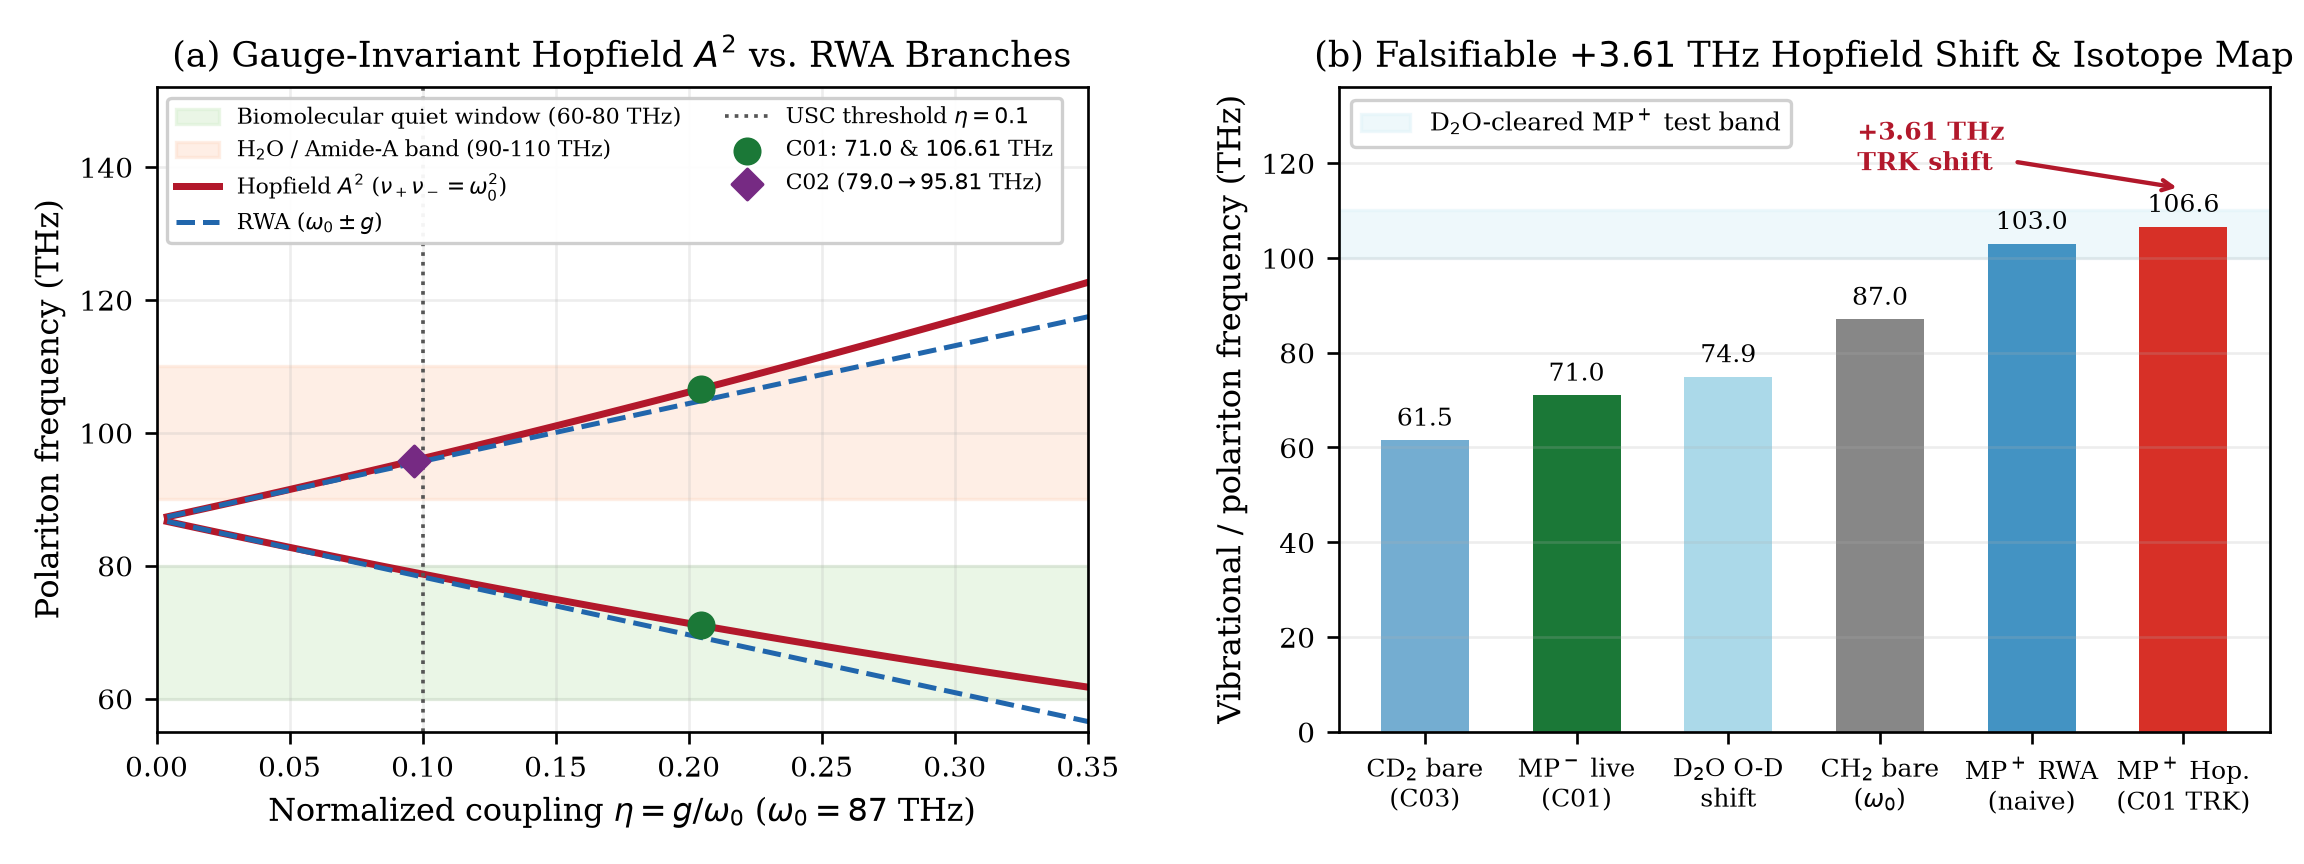
\includegraphics[width=0.78\textwidth]{figures/fig1_hopfield_a2_vs_rwa.png}
\caption{\textbf{Gauge-Invariant Hopfield $A^2$ Spectrum and Isotope Tests.} (a)~Exact Hopfield TRK polariton branches ($\nu_+\nu_-=\omega_0^2$) versus naive RWA ($\omega_0\pm g$) across $\eta = g/\omega_0$, with live certified witnesses \texttt{C01} ($\eta=0.2046$, USC) and \texttt{C02}. (b)~Direct $+3.61$~THz blue-shift of $\mathrm{MP}^+$ ($106.61$ vs.\ $103$~THz) exposed when $\text{D}_2\text{O}$ shifts water absorption to $74.9$~THz.}
\label{fig:fig1}
\end{figure*}

\begin{figure*}[t]
\centering
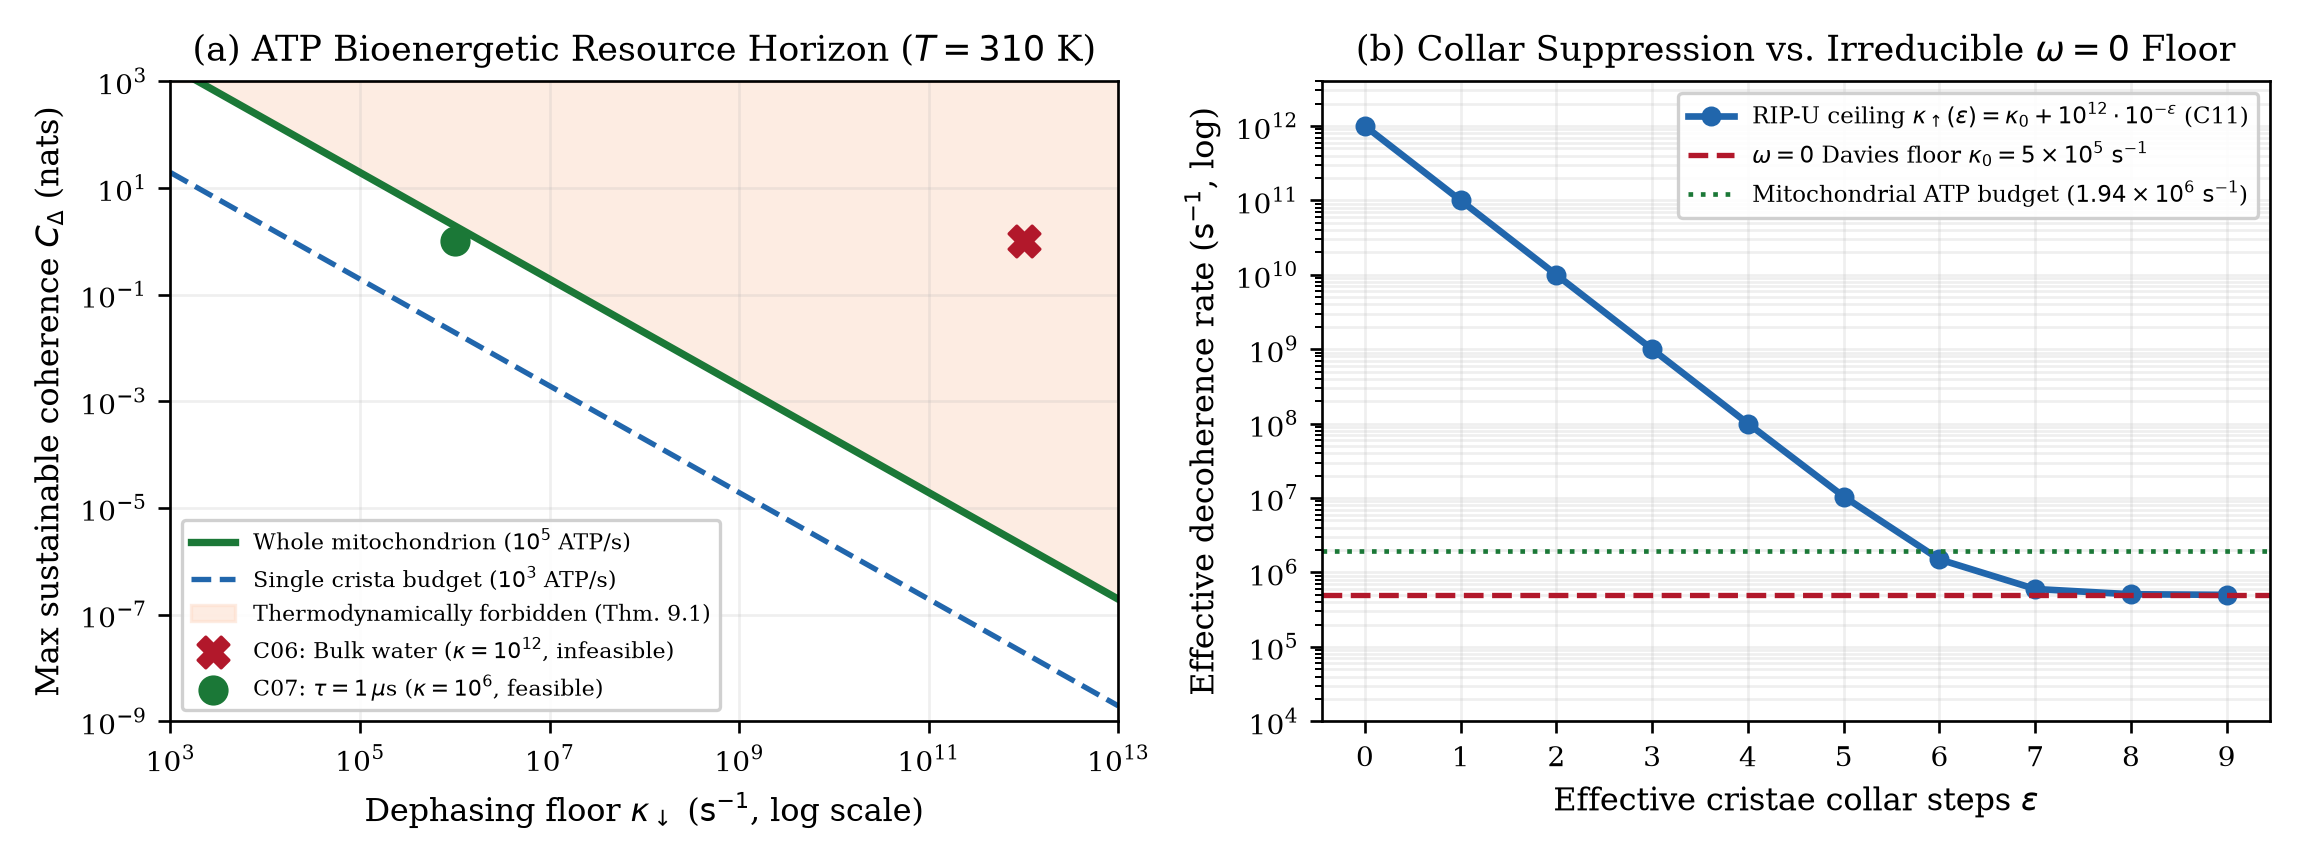
\includegraphics[width=0.78\textwidth]{figures/fig2_resource_horizon_and_rip_u.png}
\caption{\textbf{Bioenergetic ATP Resource Horizon and Cristae Collar Suppression.} (a)~Exact log-log feasibility phase diagram from Theorem~9.1 at $T=310$~K comparing whole-mitochondrion ($10^5$~ATP/s) and single-crista budgets against bulk-water dephasing (\texttt{C06}, infeasible by $5\times 10^5$) and microsecond-suppressed Regime~II (\texttt{C07}, feasible). (b)~\textsc{rip-u} geometric collar decay hitting an irreducible $\omega=0$ Davies floor (\texttt{C11}).}
\label{fig:fig2}
\end{figure*}

\begin{figure*}[t]
\centering
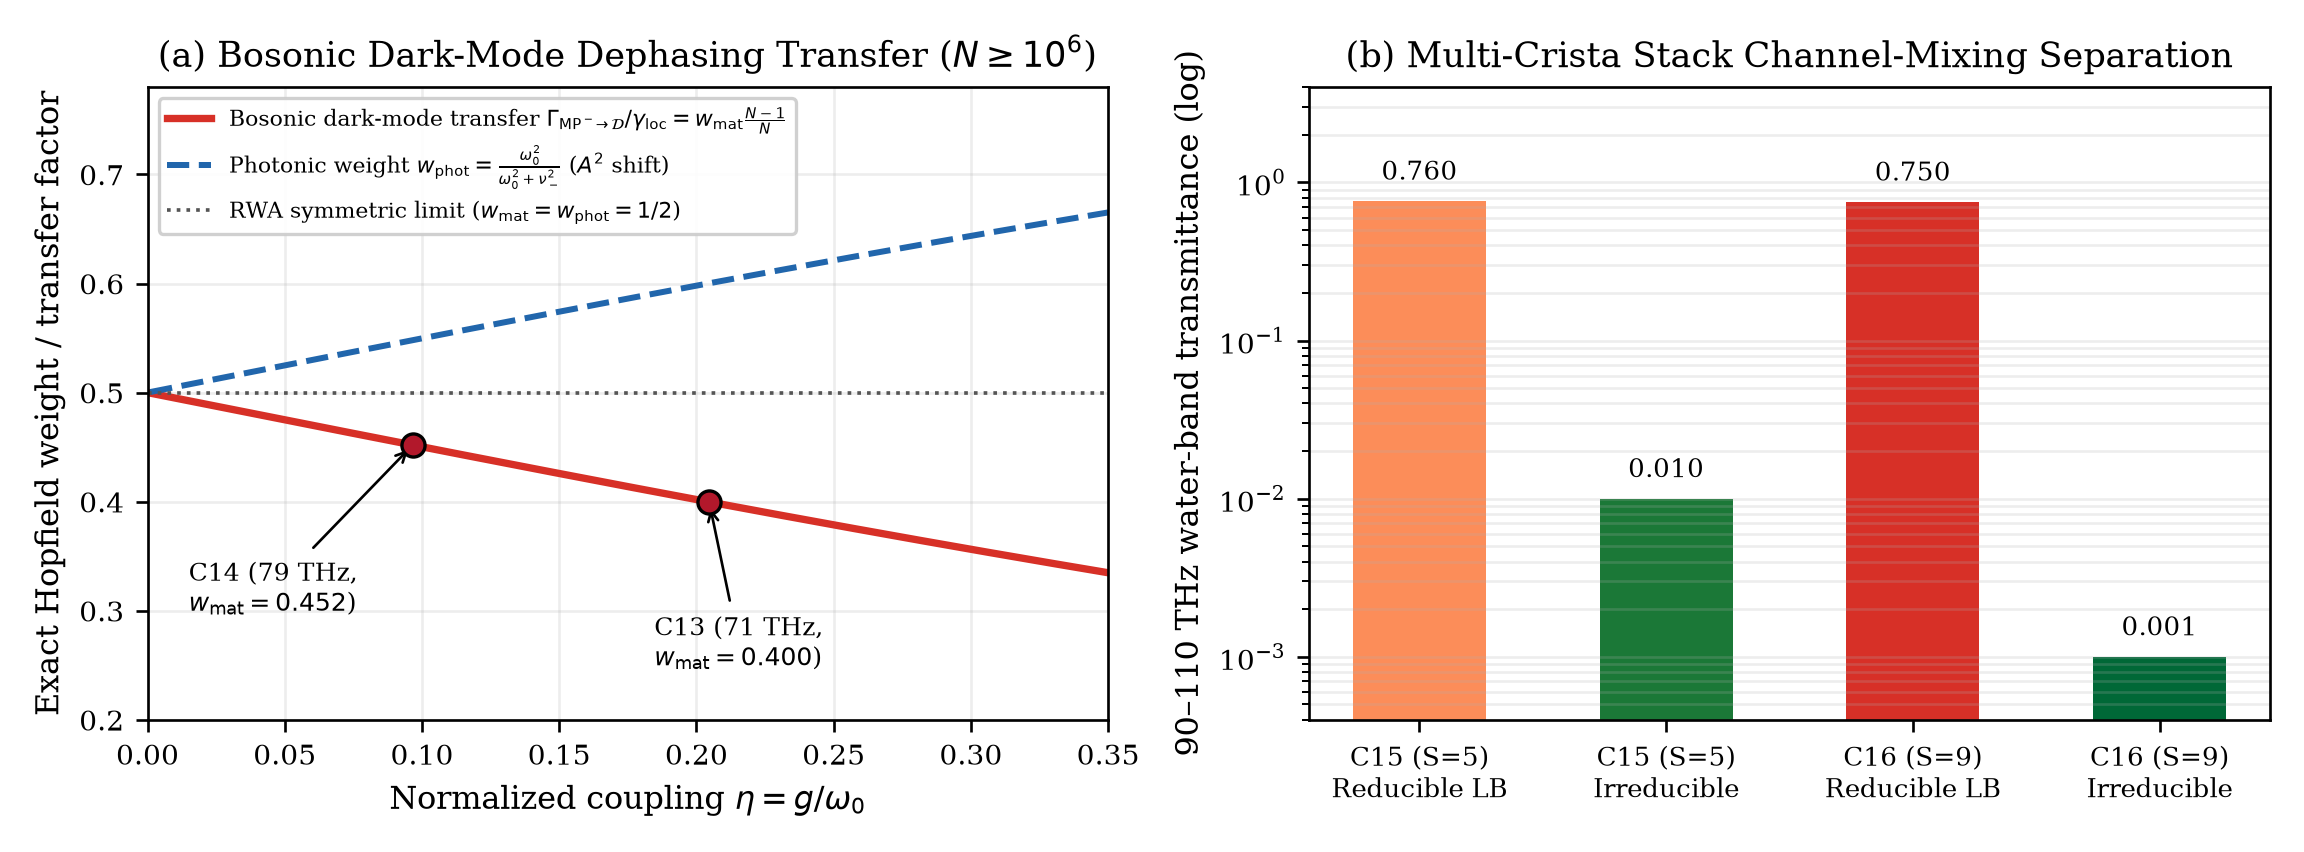
\includegraphics[width=0.78\textwidth]{figures/fig3_dark_mode_and_passive_network.png}
\caption{\textbf{Bosonic Dark-Mode Dephasing Transfer and Multi-Crista Stack Shielding.} (a)~Exact Hopfield lower-polariton matter weight $w_{\mathrm{mat}} = \nu_-^2/(\omega_0^2+\nu_-^2)$ and dark-mode dephasing transfer $\Gamma_{\mathrm{MP}^-\to\mathcal{D}}/\gamma_{\mathrm{loc}} = w_{\mathrm{mat}}\frac{N-1}{N}$ vs.\ $\eta$, with certified witnesses \texttt{C13} ($71$~THz) and \texttt{C14} ($79$~THz). (b)~Live Mode~4b water-band transmittance separation between factorized single-bilayer filters and irreducible coupled $S$-lamella cristae stacks (\texttt{C15}, \texttt{C16}).}
\label{fig:fig3}
\end{figure*}

\section{Experimental Falsification Matrix}
Table~\ref{tab:falsify} upgrades Section~11 of~\cite{Eriksson2025GeometryMembranes} into four concrete experiments decisively discriminating classical artifacts ($H_0$), passive vacuum-dressed polaritons ($H_1$: Regime~I, $C_\Delta=0$), and actively maintained quantum coherence ($H_2$: Regime~II, $C_\Delta>0$).

\begin{table}[t]
\centering
\scriptsize
\setlength{\tabcolsep}{1.8pt}
\caption{Four-test experimental falsification matrix separating $H_0$ (artifact), $H_1$ (Regime~I passive polariton), and $H_2$ (Regime~II active coherence).}
\label{tab:falsify}
\begin{tabular}{@{}llll@{}}
\toprule
Protocol & $H_0$ (Artifact) & $H_1$ ($C_\Delta=0$) & $H_2$ ($C_\Delta>0$) \\
\midrule
$\text{D}_2\text{O}$ FTIR & No $106.6$ peak & $\mathrm{MP}^+$ $106.6\pm 0.5$ & $\mathrm{MP}^+$ $106.6\pm 0.5$ \\
$\text{CD}_2$ lipid & Unshifted $71$ & $\nu_-\to 56$--$58$ & $\nu_-\to 56$--$58$ \\
2D-IR/$\Delta\Psi_m$ & No echo & Pure $T_1$/inhom. & $T_2^*\ge 0.5\,\mu\mathrm{s}$ \\
Oligomycin & Unchanged & Persists (intact) & Drops w/ ATP \\
\bottomrule
\end{tabular}
\end{table}

\section{Reproducibility and Availability}
All source code, Lean~4 proofs, certificates, figure scripts, and SHA-256 manifest (\texttt{MANIFEST.sha256}) are archived at \nolinkurl{https://github.com/lluiseriksson/mito-polariton-resource-boundary-certificates} under MIT (code/Lean/data) and CC-BY-4.0 (manuscript/figures) licenses. Reproduction requires three commands: \texttt{(cd lean \&\& lake build)}, \texttt{python -m} \nolinkurl{src.mito_polariton_bound_verifier} \texttt{certificates}, and \texttt{pytest -q}.

\paragraph{AI Assistance Disclosure.}
Google Antigravity assisted with Lean~4 proof engineering, zero-float verifier implementation, test/figure automation, and LaTeX drafting. The author verified every mathematical derivation, Lean axiom audit, certificate check, and visual figure inspection, and takes full responsibility for all contents.

\bibliographystyle{plain}
\bibliography{references}
\end{document}
